\begin{flushleft}
Per comprendere appieno il pericolo delle entità esterne, è importante prima capire che cos'è un'entità. Le entità sono variabili XML a cui è possibile fare riferimento dall'applicazione. Gli sviluppatori utilizzano le entità per definire i valori e utilizzano tali valori nel codice futuro.
\end{flushleft}

\begin{flushleft}
Esempio di entità:
\end{flushleft}

\begin{lstlisting}[language=XML]
<?xml version="1.0"?>
<!DOCTYPE example [
    <!ENTITY hello "Hello world!">
]>
<User>
    <Name>Admin</Name>
    <DisplayName>Administrator</DisplayName>
    <Message>&hello;</Message>
</User>
\end{lstlisting}

\begin{flushleft}
In questo esempio, il contenuto del tag "Message" verrà popolato dall'entità "hello" appena definita.
\end{flushleft}

\begin{flushleft}
Allora cosa sono le \textbf{entità esterne}?
\end{flushleft}

\begin{flushleft}
Sono fondamentalmente la stessa cosa, tuttavia consentono di definire entità con dati esterni, mentre con le entità normali occorre definire esplicitamente i dati che vengono archiviati.
\end{flushleft}

\begin{flushleft}
Per creare un'entità esterna, occorre utilizzare la parola chiave "SYSTEM", seguita da un URL, che indicherà all'applicazione di recuperare il contenuto da quella risorsa esterna.
\end{flushleft}

\begin{flushleft}
Esempio di entità esterna:
\end{flushleft}

\begin{lstlisting}[language=XML]
<?xml version="1.0"?>
<!DOCTYPE example [
    <!ENTITY hello SYSTEM "https://www.google.com/robots.txt">
]>
<User>
    <Name>Admin</Name>
    <DisplayName>Administrator</DisplayName>
    <Message>&hello;</Message>
</User>
\end{lstlisting}

\begin{flushleft}
Questo frammento recupererà i contenuti dall'URL fornito e li memorizzerà nell'entità "hello". La cosa interessante delle entità esterne è che non si è limitati alle risorse "esterne".
\end{flushleft}

\begin{flushleft}
Utilizzando diversi protocolli URI, possiamo interagire con altre risorse. Se vogliamo leggere un file locale del server o del PC della vittima, possiamo usare il seguente URI.
\end{flushleft}

\begin{flushleft}
file:///etc/passwd
\end{flushleft}

\begin{flushleft}
Ora che abbiamo ottenuto il contenuto del file archiviato in una variabile, possiamo creare un'altra entità esterna per inviare una richiesta al nostro server malevolo con i contenuti. Una volta inviata la richiesta al nostro server, possiamo controllare i log di accesso e osservare il contenuto del file.
\end{flushleft}

\begin{flushleft}
\textbf{Panoramica sull'exploit}
\end{flushleft}


\begin{flushleft}
Affinché un utente malintenzionato possa sfruttare con successo questa vulnerabilità, dovrebbe convincere una vittima ad aprire un file MTZ o MTGL all'interno di Maltego. Questo è abbastanza comune poiché Maltego utilizza questi file per memorizzare il grafo e le varie impostazioni di progetto.
\end{flushleft}

\begin{flushleft}
Ad esempio, i file MTGL/MTGX sono essenzialmente file di progetto.
\end{flushleft}

\begin{flushleft}
I file MTZ, tuttavia, sono usati esclusivamente per le configurazioni, come nuove transform, nuove entità, ecc.
\end{flushleft}

\begin{flushleft}
\textbf{Panoramica tecnica}
\end{flushleft}

\begin{flushleft}
Per questo esempio useremo un file di grafo perché questi sono i meno sospettabili e sono spesso condivisi tra altre persone. Il primo passaggio consiste nel creare un file di grafo vuoto e trascinare un'entità nella vista. Fatto ciò, possiamo salvarlo e iniziare a modificare le cose all'interno del file MTGL.
\end{flushleft}

\begin{flushleft}
La prima cosa che si nota riguardo i file MTGL/MTZ è che in realtà sono semplicemente un insieme di file XML e di file di proprietà, compressi in un archivio ZIP. Questo rende molto semplice il "reverse engineering" dei formati di file di Maltego.
\end{flushleft}

\begin{flushleft}
Ecco uno screenshot che mostra il file MTGL su cui faremo l'esperimento:

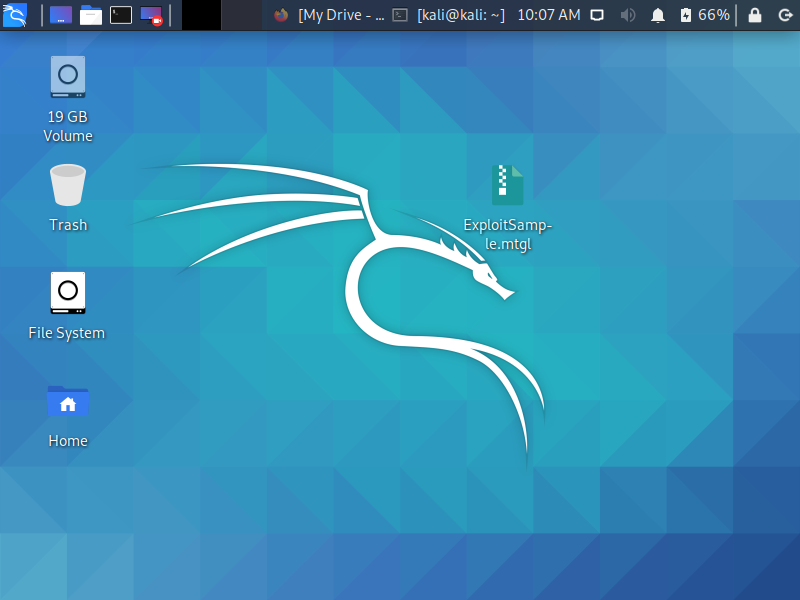
\includegraphics[scale=0.5]{images/Screenshot-file-MTGL-Maltego.png}
\end{flushleft}

\begin{flushleft}
Ecco quello che accade se decomprimiamo il file ExploitSample.mtgl:

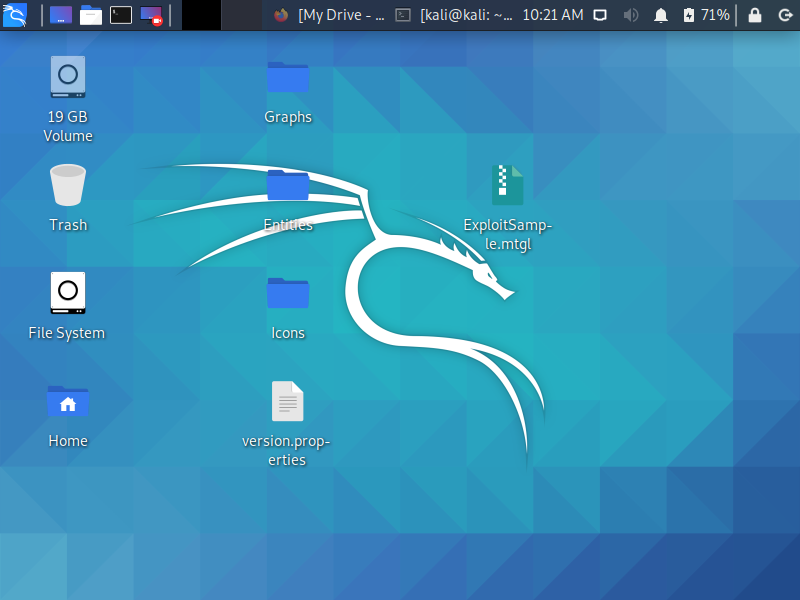
\includegraphics[scale=0.5]{images/Screenshot cartelle interne file MTGL.png}
\end{flushleft}

\begin{flushleft}
Il file MTGL contiene dunque 3 cartelle, Graphs, Entities e Icons, ed un file denominato version.properties.
\end{flushleft}

\begin{flushleft}
L'idea qui è di modificare uno dei file XML e aggiungere il nostro payload, per poi reimpacchetare il file MTGL per inviarlo alla vittima.
\end{flushleft}

\begin{flushleft}
In questo esempio modificheremo una delle entità, che di default è simile alla seguente:
\end{flushleft}

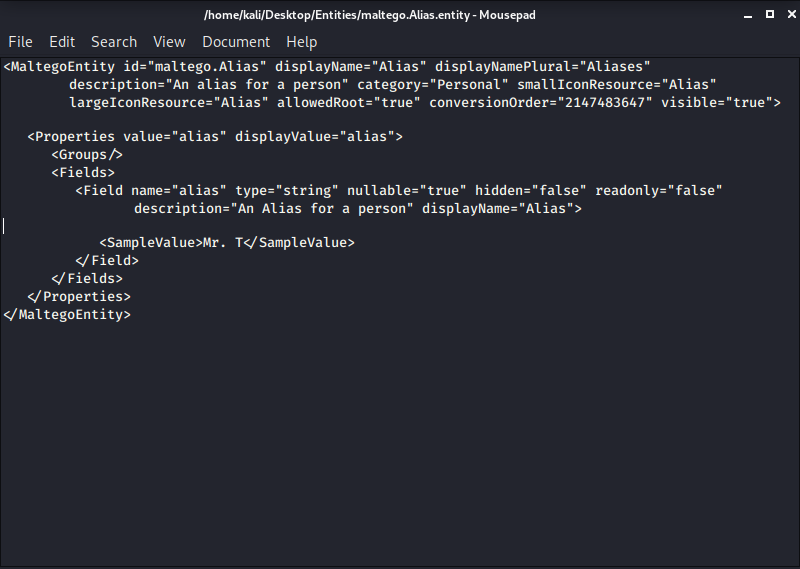
\includegraphics[scale=0.5]{images/Screenshot-file-maltego.Alias.entity.png}

\begin{flushleft}
Tutto ciò che dobbiamo fare è aggiungere un'entità, quindi fare in modo che faccia riferimento a un altra entità esterna che sarà responsabile dell'esfiltrazione.
\end{flushleft}

\begin{flushleft}
Ecco il file con l'aggiunta del payload:
\end{flushleft}

\includegraphics[scale=0.5]{images/Screenshot file entità con payload.png}

\begin{flushleft}
Ed ecco il contenuto del file lol.dtd:
\end{flushleft}

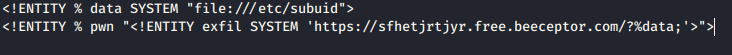
\includegraphics[scale=0.5]{images/Screenshot file lol.dtd.png}

\begin{flushleft}
Per ragioni di test, verrà usato beeceptor.com, che è principalmente usato per REST API mocking. Beeceptor ci consente di settare delle regole mock API, permettendoci di hostare lì il contenuto del file letto dalla macchina vittima.
\end{flushleft}

\begin{flushleft}
Ad alto livello, ecco come funziona il payload. Innanzitutto, creiamo un'entità che acquisisca il contenuto del file lol.dtd dall'URL fornito.
\end{flushleft}

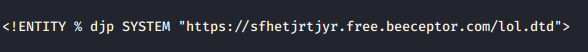
\includegraphics[scale=0.6]{images/Screenshot_1.png}

\begin{flushleft}
Quindi, nel file lol.dtd, creiamo un'altra entità che acquisisca il contenuto del file locale scelto.
\end{flushleft}

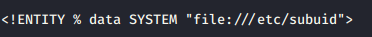
\includegraphics[scale=0.5]{images/Screenshot_2.png}

\begin{flushleft}
Infine, definiamo un'altra entità, che invierà una richiesta GET con i contenuti dell'entità "data" che abbiamo creato. Essenzialmente stiamo esfiltrando il contenuto del file.
\end{flushleft}

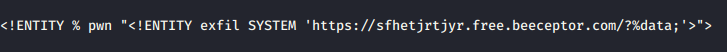
\includegraphics[scale=0.5]{images/Screenshot_3.png}

\begin{flushleft}
Ora, quando Maltego tenta di eseguire il rendering dell'entità, il tag SampleValue avrà come valore quello dell'entità esterna "exfil":
\end{flushleft}

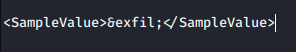
\includegraphics[scale=0.7]{images/Screenshot_4.png}

\begin{flushleft}
Il parser XML leggerà la definizione della nostra entità "exfil", valutando in definitiva le nostre entità istantaneamente quando viene eseguito il rendering del file grafico.
\end{flushleft}

\begin{flushleft}
Ora che abbiamo compreso come funziona l'attacco, possiamo andare avanti e testarlo. Creiamo un semplice file di grafo come è stato fatto vedere precedentemente. Una volta che abbiamo fatto, possiamo decomprimere il file col seguente comando:
\end{flushleft}

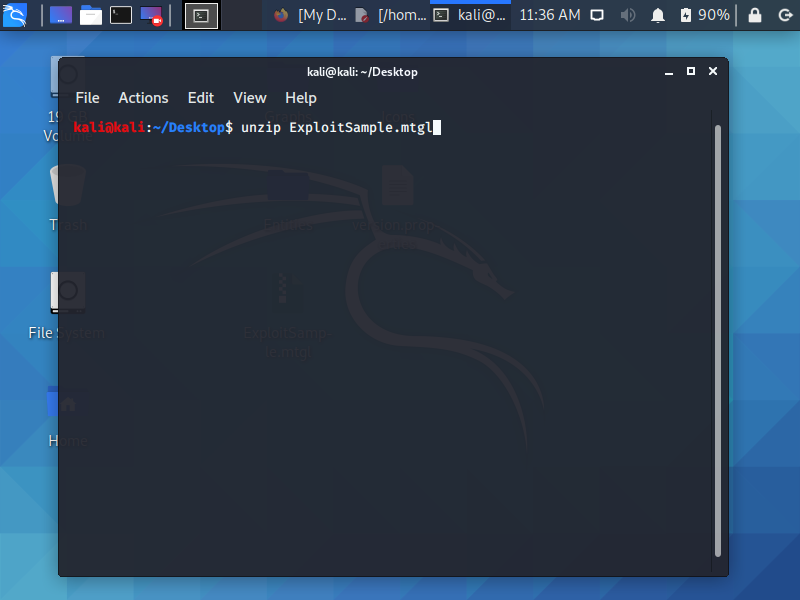
\includegraphics[scale=0.4]{images/Screenshot unzip file MTGL.png}

\begin{flushleft}
Ora possiamo modificare il file "Entities/maltego.Alias.entity", con i seguenti contenuti:
\end{flushleft}

\includegraphics[scale=0.4]{images/Screenshot file entità con payload.png}

\begin{flushleft}
Dobbiamo anche impostare la regola su beeceptor, affinché alla ricezione di una richiesta HTTP di tipo GET del file lol.dtd, il nostro server restituisca in risposta il contenuto del file.
\end{flushleft}

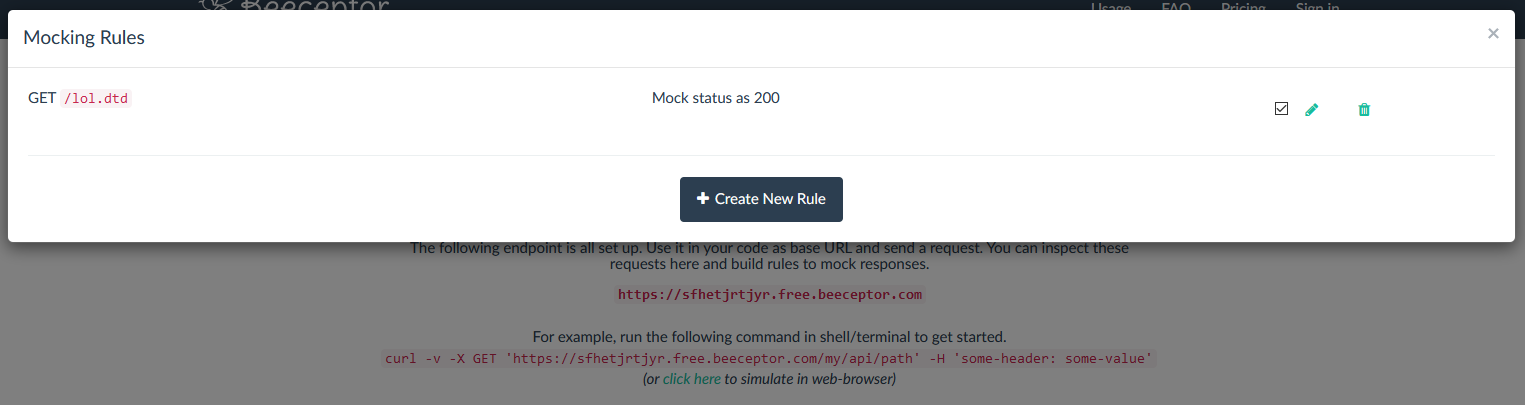
\includegraphics[scale=0.4]{images/Screenshot Beeceptor.png}

\begin{flushleft}
Impostiamo la regola in modo che la richiesta GET a lol.dtd serva il seguente contenuto:
\end{flushleft}

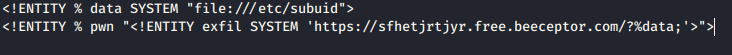
\includegraphics[scale=0.4]{images/Screenshot file lol.dtd.png}


\begin{flushleft}
Ora che abbiamo eseguito tutta la configurazione, tutto ciò che dobbiamo fare è reimpacchetare/comprimere il file MTGL e inviarlo alla vittima (nel nostro esperimento, siamo noi stessi ad impersonare la vittima e ad aprire il file payload.mtgl).
\end{flushleft}


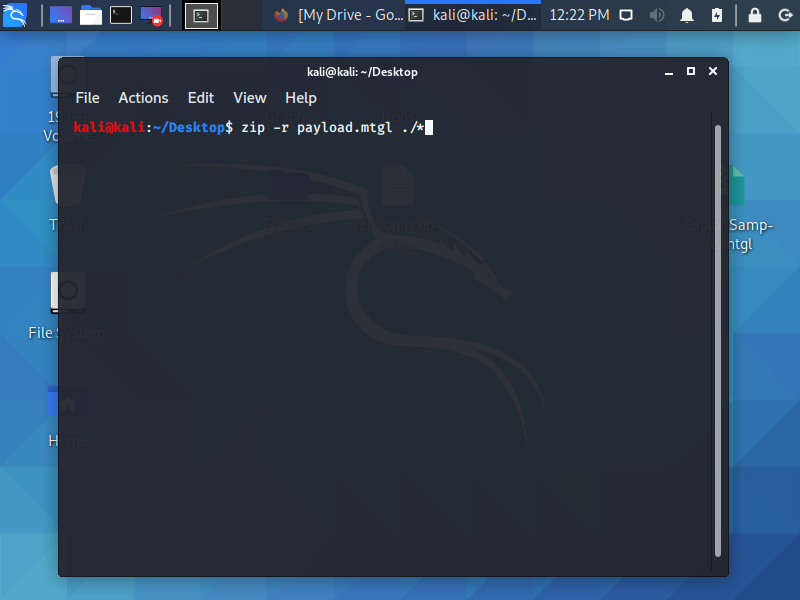
\includegraphics[scale=0.4]{images/Screenshot zip file MTGL.png}

\begin{flushleft}
Provando ad aprire il file payload.mtgl con Maltego, vedremo che su Beeceptor, in particolare su https://sfhetjrtjyr.free.beeceptor.com, comparirà il contenuto del file /etc/subuid. L'attacco ha dunque avuto l'effetto atteso.
\end{flushleft}
